\documentclass{article}
\usepackage[utf8]{inputenc}
\usepackage{graphicx}
\usepackage{titlepic}
\usepackage{hyperref}
\usepackage{xcolor}
\usepackage{amsmath}


\titlepic{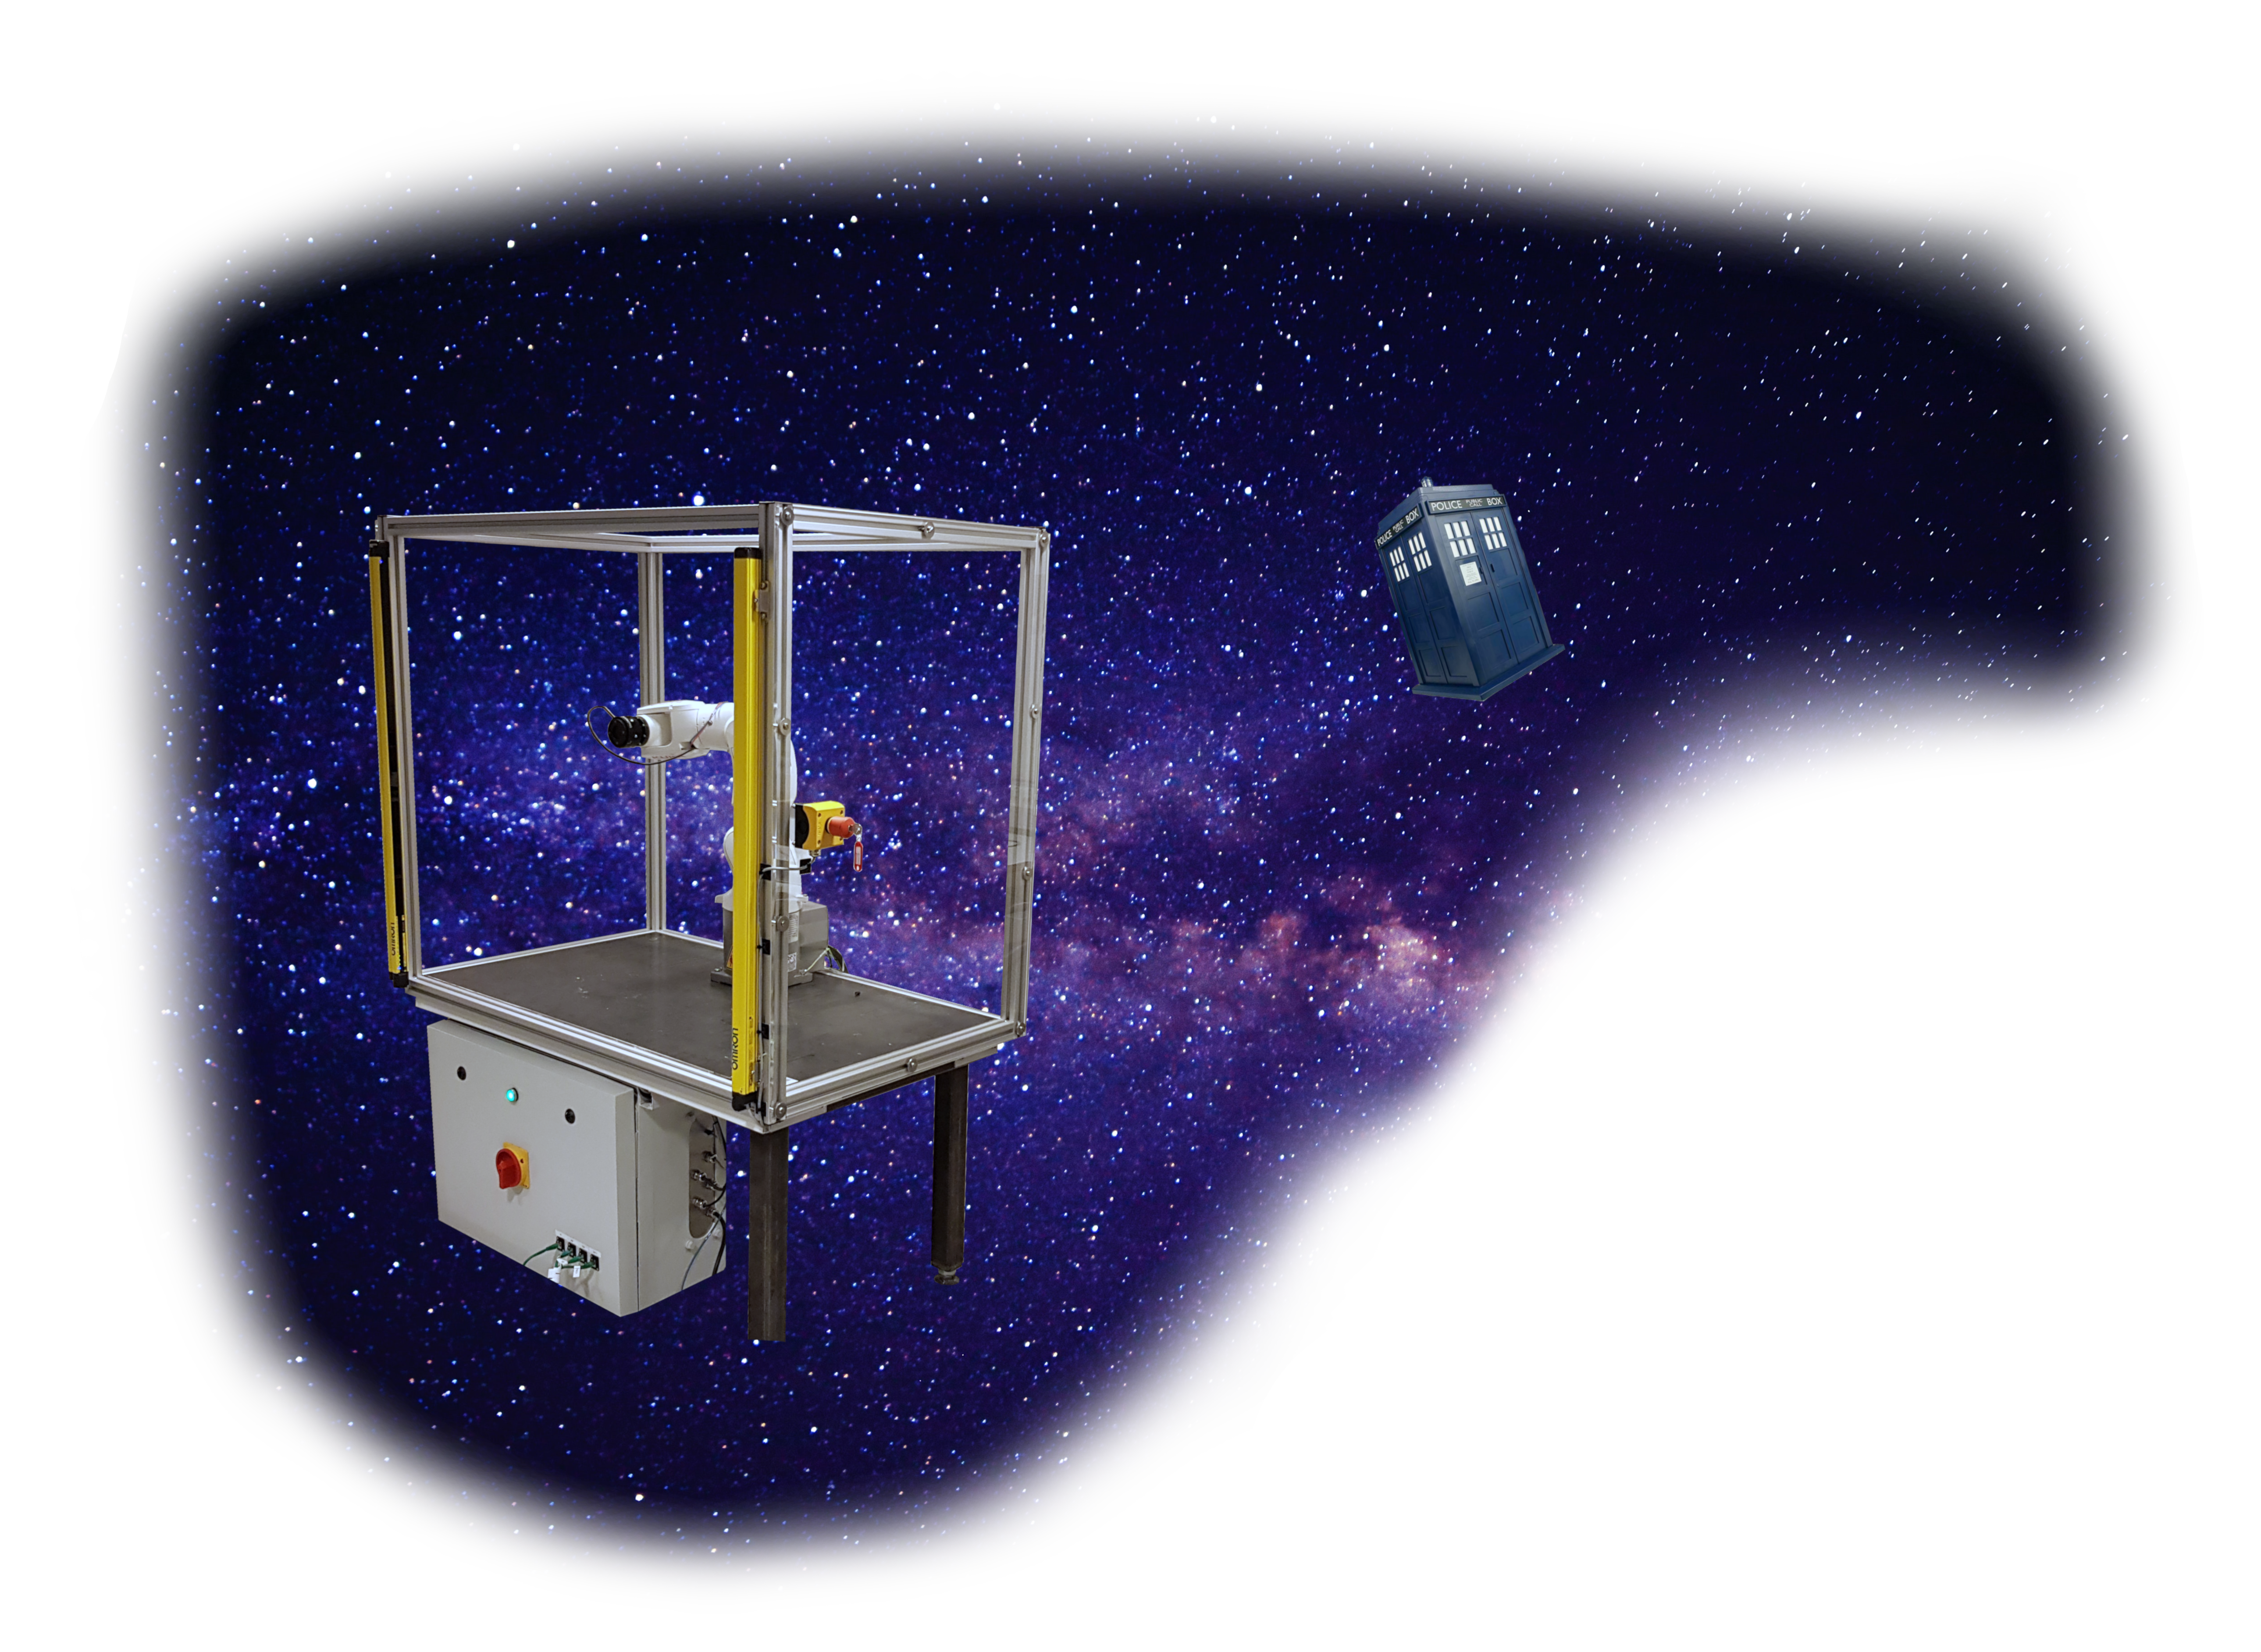
\includegraphics[width=\textwidth]{Pictures/robotlab1_final.png}}
\title{Getting started with Kuka Robot Cell}
\author{Espen Teigen }
\date{March 2019}


\begin{document}

\maketitle

    Github: https://github.com/EspenTeigen/Kuka-KR-C4-commissioning

\newpage
\tableofcontents{}
\newpage

\section{Overview of the Robot-cell and it's parts}
    \subsection{Manipulator}
        \subsubsection{Force-torque sensor}
        \subsubsection{Pneumatic's}

    \subsection{Robot Controller}
        \subsubsection{PC-interface}
        \paragraph{Software}
        \subsubsection{EtherCAT}


    \subsection{Control cabinet}
        \subsubsection{Front panel}
        \subsubsection{PLC}
        \paragraph{PC-interface}
        \paragraph{Software}
        \subsubsection{Pneumatic's}
    
    \subsection{Safety}
        \subsubsection{Do's and dont's }
        \subsubsection{Emergency stop's}
        \subsubsection{Light grid}


\end{document}
